\documentclass{beamer}
%\documentclass[handout]{beamer}

% language settings
%\usepackage{fontspec, polyglossia}
%\setdefaultlanguage{magyar}

% common packages
\usepackage{amsmath, multimedia, hyperref, color, multirow}
%\usepackage{graphicx}
\usepackage{pifont}

% TikZ
\usepackage{tikz}
\usetikzlibrary{arrows.meta, decorations.pathmorphing, decorations.pathreplacing, shapes.geometric,mindmap}
\usetikzlibrary{shapes.geometric,fadings,bayesnet}

% beamer styles
\mode<presentation>{
\usetheme{Warsaw}
%\usetheme{Antibes}
\usecolortheme{beaver}
%\usecolortheme{seahorse}
%\usefonttheme{structureitalicserif}
\setbeamercovered{transparent}
}
\setbeamertemplate{blocks}[rounded][shadow=true]
\AtBeginSubsection[]{
  \begin{frame}<beamer>{Contents}
  \end{frame}
}
%\useoutertheme[]{tree}

% title, etc
%\title{Drug Repurposing to Alzheimer's Disease Using TWAS and the PPI Network}
\title{Drug Repurposing to Alzheimer's Disease}
\author{Attila Jones}
\date{National Institute of Health}

\begin{document}

\maketitle

\section{Introduction}

\begin{frame}{Drug repurposing}
\begin{columns}[t]
\begin{column}{0.6\textwidth}

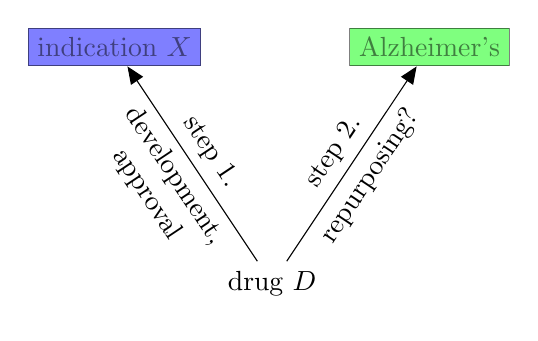
\begin{tikzpicture}
\path (0,0) node (drug) {drug $D$}
	(-2,3) node[draw,fill=blue,semitransparent] (ind) {indication $X$}
	( 2,3) node[draw,fill=green,semitransparent] (alz) {Alzheimer's};
\path[->] (drug) edge node[below,sloped,text width=3cm,text centered] {development, approval} node[above,sloped]
	{step 1.} (ind);
\path[->] (drug) edge node[below,sloped] {repurposing?} node[above,sloped]
	{step 2.} (alz);
\end{tikzpicture}
\end{column}

\begin{column}{0.4\textwidth}
Approaches to repurposing
\begin{enumerate}
\item shared gene\\
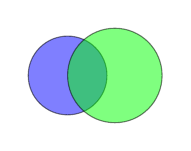
\begin{tikzpicture}
\draw[fill=blue,semitransparent] (0,0) circle (0.5cm);
\draw[fill=green,semitransparent] (0.6,0) circle (0.6cm);
\end{tikzpicture}
\item network based
\begin{description}
	\tiny
\item[Guney,..., Barabási 2016] proximity
\item[Cheng,..., Barabási 2018] validation
\end{description}
\end{enumerate}
\end{column}
\end{columns}
\end{frame}

\begin{frame}{The network based approach}%{Where the shared gene approach fails}
\begin{columns}[t]
\begin{column}{0.35\textwidth}
\begin{center}
PPI toy network

\tiny
Alzheimer's genes:
\tikz{\node[white,circle,inner sep=1pt,fill=red] {B}}
\tikz{\node[white,circle,inner sep=1pt,fill=red] {D}}
\tikz{\node[white,rectangle,inner sep=2.5pt,fill=red] {E}}
\end{center}

\includegraphics[width=\columnwidth]{../../../results/2021-06-14-proximity/toy-proximal-arrow.png}
\end{column}

\begin{column}{0.65\textwidth}

\begin{center}
Applicability
\end{center}
\begin{tabular}{r|c|c|}
\footnotesize
\hline
& \multicolumn{2}{c|}{approach} \\
& shared gene & network based \\
\hline
drug $\rightarrow$ \tikz{\node[white,rectangle,inner sep=2.5pt,fill=red] {E}}& \ding{52} & \ding{52}\ding{52}  \\
drug $\rightarrow$ \tikz{\node[white,rectangle,inner sep=2.5pt,fill=blue] {J}} & \ding{56} & \ding{52}\ding{52} \\
\hline
\end{tabular}
\vfill
\begin{center}
Network based proximity
\end{center}
\begin{description}
\footnotesize
\item[raw distance] \( d = \frac{1}{|T|}\sum_{t \in T} \min_{s \in S} d(s, t)
	= \frac{1}{2} \)
\item[standardized] \(z = -0.454, \; p = 0.324\)

\end{description}
\end{column}
\end{columns}
\end{frame}

\begin{frame}{A case study in the real PPI network}{Input data}
\begin{columns}[t]
\begin{column}{0.5\textwidth}

\begin{center}
three AD gene sets
\end{center}

\includegraphics[width=1.0\columnwidth]{../../../notebooks/2021-08-04-guney-tools/named-figure/AD-gene-sets-venn3.pdf}
\end{column}

\begin{column}{0.5\textwidth}

\begin{center}
two ``target'' gene sets
\end{center}
	\footnotesize
\begin{tabular}{ccc}
name & genes & drug \\
\hline
HCQ targets & TLR7, TRL9 & HCQ \\
2AD genes & ABCA7, APOE  & none \\
\end{tabular}
\end{column}
\end{columns}
\begin{center}
Goal: evaluate proximity for each target and AD gene set
\end{center}
\end{frame}

\begin{frame}{A case study in the real PPI network}{Results}
\includegraphics[width=1.0\textwidth]{../../../notebooks/2021-08-04-guney-tools/named-figure/proximity-d-z-p.pdf}
\end{frame}

\begin{frame}{High confidence AD gene sets}
\begin{columns}[t]
\begin{column}{0.5\textwidth}

\includegraphics[width=1.0\textwidth]{../../../notebooks/2021-07-01-high-conf-ADgenes/named-figure/knowledge-twas-proteo-venn.pdf}
\end{column}

\begin{column}{0.5\textwidth}

\end{column}
\end{columns}
\end{frame}

\begin{frame}{Extending high confidence set with more AD genes}
	{Candidate AD gene prioritization with, e.g., Endeavour}
\includegraphics[width=\textwidth]{figures/from-others/endeavour-2016-Fig1.jpg}

\vfill
\tiny Tranchevent et al 2016
\end{frame}

\end{document}


\begin{columns}[t]
\begin{column}{0.5\textwidth}

\end{column}

\begin{column}{0.5\textwidth}

\end{column}
\end{columns}
